% $Header$

\documentclass{beamer}
% common for paper and presentation

%%-- My stuff

\usepackage{pdfpages}[interpolate=false]
\usepackage{amsmath,amsfonts,amsthm}
\usepackage{mathtools,bm}
\usepackage{listings,color}
\usepackage{tikz,float}
\usepackage[font=small]{caption}
\usetikzlibrary{arrows,snakes,backgrounds}
%funk for externalizing graphics...
%\pgfrealjobname{thesis}


\newcommand{\lstVecMat}{\lstinputlisting[firstline=10, firstnumber=10, lastline=11]{../cpp/include/common.h}}
\newcommand{\lstVPoly}{\lstinputlisting[firstline=13, firstnumber=13, lastline=16]{../cpp/include/common.h}}
\newcommand{\lstD}{\lstinputlisting[firstline=20, firstnumber=20, lastline=20]{../cpp/include/common.h}}
\newcommand{\lstIstream}{\lstinputlisting[firstline=22, firstnumber=22, lastline=25]{../cpp/include/common.h}}
\newcommand{\lstOstream}{\lstinputlisting[firstline=26, firstnumber=26, lastline=29]{../cpp/include/common.h}}
\newcommand{\lstInputError}{\lstinputlisting[firstline=30, firstnumber=30, lastline=30]{../cpp/include/common.h}}
\newcommand{\lstUsage}{\lstinputlisting[firstline=36, firstnumber=36, lastline=36]{../cpp/include/common.h}}
\newcommand{\lstTranspose}{\lstinputlisting[firstline=41, firstnumber=41, lastline=41]{../cpp/include/common.h}}
\newcommand{\lstProjectM}{\lstinputlisting[firstline=44, firstnumber=44, lastline=44]{../cpp/include/common.h}}
\newcommand{\lstCheckEmpty}{\lstinputlisting[firstline=129, firstnumber=129, lastline=131]{../cpp/src/common.cpp}}
\newcommand{\lstFME}{\lstinputlisting[firstline=166, firstnumber=166, lastline=183]{../cpp/src/common.cpp}}
\newcommand{\lstFMEPart}{\lstinputlisting[firstline=169, firstnumber=169, lastline=172]{../cpp/src/common.cpp}}
\newcommand{\lstFMEMove}{\lstinputlisting[firstline=174, firstnumber=174, lastline=174]{../cpp/src/common.cpp}}
\newcommand{\lstFMEConvolute}{\lstinputlisting[firstline=176, firstnumber=176, lastline=181]{../cpp/src/common.cpp}}
\newcommand{\lstLiftHcone}{\lstinputlisting[firstline=13, firstnumber=13, lastline=13]{../cpp/include/hcone.h}}
\newcommand{\lstIntersectVCone}{\lstinputlisting[firstline=53, firstnumber=53, lastline=59]{../cpp/src/hcone.cpp}}
\newcommand{\lstHconeToVcone}{\lstinputlisting[firstline=63, firstnumber=63, lastline=69]{../cpp/src/hcone.cpp}}
\newcommand{\lstLiftVcone}{\lstinputlisting[firstline=9, firstnumber=9, lastline=9]{../cpp/include/vcone.h}}
\newcommand{\lstProjectHCone}{\lstinputlisting[firstline=51, firstnumber=51, lastline=57]{../cpp/src/vcone.cpp}}
\newcommand{\lstVconeToHcone}{\lstinputlisting[firstline=61, firstnumber=61, lastline=67]{../cpp/src/vcone.cpp}}
\newcommand{\lstProjectZero}{\lstinputlisting[firstline=12, firstnumber=12, lastline=16]{../cpp/src/polyhedra.cpp}}
\newcommand{\lstNormalizeP}{\lstinputlisting[firstline=20, firstnumber=20, lastline=30]{../cpp/src/polyhedra.cpp}}
\newcommand{\lstHpolyToHCone}{\lstinputlisting[firstline=34, firstnumber=34, lastline=42]{../cpp/src/polyhedra.cpp}}
\newcommand{\lstHconeToHPoly}{\lstinputlisting[firstline=46, firstnumber=46, lastline=54]{../cpp/src/polyhedra.cpp}}
\newcommand{\lstVpolyToVCone}{\lstinputlisting[firstline=59, firstnumber=59, lastline=74]{../cpp/src/polyhedra.cpp}}
\newcommand{\lstVconeToVPoly}{\lstinputlisting[firstline=78, firstnumber=78, lastline=92]{../cpp/src/polyhedra.cpp}}
\newcommand{\lstHpolyToVPoly}{\lstinputlisting[firstline=96, firstnumber=96, lastline=98]{../cpp/src/polyhedra.cpp}}
\newcommand{\lstVpolyToHPoly}{\lstinputlisting[firstline=100, firstnumber=100, lastline=102]{../cpp/src/polyhedra.cpp}}


\renewcommand{\vec}[1]{\mathbf{#1}}
\newcommand{\set}[1]{\left\{#1\right\}}
\DeclareMathOperator{\cone}{cone}
\DeclareMathOperator{\conv}{conv}
\DeclareMathOperator{\VLift}{T_V}
\DeclareMathOperator{\HLift}{T_H}
\newcommand{\ip}[2]{\left\langle #1, #2 \right\rangle}

%special letters
\newcommand{\R}{\mathbb{R}}
\newcommand{\0}{\vec{0}}
\newcommand{\1}{\vec{1}}
\renewcommand{\r}{\vec{r}}
\renewcommand{\u}{\vec{u}}
\newcommand{\x}{\vec{x}}
\newcommand{\y}{\vec{y}}
\newcommand{\z}{\vec{z}}
\newcommand{\e}{\vec{e}}
\newcommand{\w}{\vec{w}}
\renewcommand{\t}{\vec{t}}
\renewcommand{\v}{\vec{v}}
\renewcommand{\b}{\vec{b}}
\newcommand{\faij}{\forall i\in P,\forall j \in N}
\newcommand{\blambda}{\bm{\lambda}}
\newcommand{\bsigma}{\bm{\sigma}}
\newcommand{\bmu}{\bm{\mu}}

%symbols
\newcommand{\st}{\;|\;}
\newcommand{\St}{\;\Big|\;}

%constants
\newcommand{\Udim}{p}
\newcommand{\Vdim}{n}
\newcommand{\Adim}{m}
\newcommand{\mspaceA}{\R^{{\Adim}\times d}}
\newcommand{\mspaceB}{\R^{m_1\times (d+\Udim)}}
\newcommand{\mspaceC}{\R^{m_2\times (d+\Udim)}}

%matrices and vectors with domain
\newcommand{\bv}{\b \in \R^{\Adim}}
\newcommand{\tv}{\t \in \R^{\Udim}}
\renewcommand{\l}{\bm{\lambda}}
\newcommand{\lv}{\l \in \R^{\Vdim}}
\newcommand{\yv}{\y \in \R^{d+1}}
\newcommand{\xv}{\x \in \R^d}
\newcommand{\mV}{V \in \R^{d\times \Vdim}}
\newcommand{\mU}{U \in \R^{d\times \Udim}}
\newcommand{\mA}{A \in \mspaceA}
\newcommand{\mB}{B \in \mspaceB}
\newcommand{\mC}{B' \in \mspaceC}
\newcommand{\xt}{\pmb  \x\\ \t\pme }
\newcommand{\xw}{\pmb  \x\\ \w\pme }
\newcommand{\xAx}{\pmb \x\\ A\x\pme }
\newcommand{\xz}{\pmb  \x\\ \0\pme }
\newcommand{\xx}{\pmb  x_0\\ \x\pme }
\newcommand{\sxx}{\psmb  x_0\\ \x\psme }
\newcommand{\onex}{\pmb 1\\ \x\pme }
\newcommand{\zw}{\pmb  \0\\ \w\pme }
\newcommand{\eAj}{\pmb \e_j\\ A^j\pme }
\newcommand{\neAj}{\pmb -\e_j\\ -A^j\pme }
\newcommand{\ee}{\pmb  \0 \\ 1 \pme }
\newcommand{\zei}{\pmb \0 \\ \e_i \pme }
\newcommand{\lcone}{\pmb  \0 & \vec{1} \\ U & V \pme }
\newcommand{\xjp}{x_j^+}
\newcommand{\xjm}{x_j^-}
\newcommand{\Yi}{Y^i_{k}}
\newcommand{\Yj}{Y^j_{k}}
\newcommand{\Yl}{Y^l_{k}}
\newcommand{\Uiz}{U^i_{0}}
\newcommand{\Ujz}{U^j_{0}}
\newcommand{\Ulz}{U^l_{0}}
\newcommand{\Bik}{B^k_i}
\newcommand{\Bjk}{B^k_j}
\newcommand{\Blk}{B^k_l}

%sums
\newcommand{\tusum}{\sum_{1\leq j \leq \Udim}t_j U^j}
\newcommand{\lvsum}{\sum_{1\leq j \leq \Vdim}\lambda_j V^j}
\newcommand{\lsum}{\sum_{1\leq j \leq \Vdim}\lambda_j}
\newcommand{\jsum}{\sum_{1\leq j \leq d}}
\newcommand{\isum}{\sum_{1\leq i \leq n}}
\newcommand{\Psum}{\sum_{i\in P}}
\newcommand{\Nsum}{\sum_{j\in N}}
\newcommand{\Zsum}{\sum_{l\in Z}}
\newcommand{\NPsum}{\sum_{\substack{i\in P \\ j\in N}}}
\newcommand{\isconv}{\lambda_j \geq 0 \lsum = 1}
\newcommand{\sumi}{\sum\nolimits_i}
\newcommand{\sumj}{\sum\nolimits_j}

% Polyhedra
\newcommand{\HC}[1]{\set{\x\st #1\x\leq\0}}
\newcommand{\HP}[2]{\set{\x\st #1\x\leq #2}}
\newcommand{\VP}[2]{\cone(#1) + \conv(#2)}
\newcommand{\LHC}{\set{\xx\St\big[-\vec{b}|A\big]\xx\leq\0}}
\newcommand{\hpxz}{\set{\xx\St x_0 = 1}}
\newcommand{\shpxz}{\set{\sxx\st x_0 = 1}}

\usepackage{thmtools,cleveref}

%text macros
\newcommand{\MWT}{Minkowski-Weyl Theorem}
\newcommand{\texteq}[2]{\begin{equation}\text{#1}\label{#2}\end{equation}}
\newcommand{\LI}{linear-independent}

%code stuff
\newcommand{\cppSourceDir}{../../cpp}
%%
\newcommand{\smallstack}[2]{\left(\begin{smallmatrix}#1 \\ #2\end{smallmatrix}\right)}

\newcommand{\lsti}[1]{\lstinline!#1!}
\newcommand{\filename}[1]{\texttt{#1}}
\newcommand{\mli}[1]{\text{\lsti{#1}}}
\newcommand{\norm}[1]{\left|\left|#1\right|\right|}
\renewcommand{\pmb}{\begin{pmatrix*}[r]}
\newcommand{\pme}{\end{pmatrix*}}
\newcommand{\psmb}{\begin{psmallmatrix*}[r]}
\newcommand{\psme}{\end{psmallmatrix*}}

\lstset{
	language=C++,
	backgroundcolor=\color[rgb]{.9,.9,.9},
	basicstyle=\small\tt,
	keywordstyle=\color[rgb]{0,.2,1},
	commentstyle=\color[rgb]{0,.6,.2},
	numbers=left,
	showstringspaces=false
}

%max bound
\newcommand{\MX}{10}
%draw the grid 
\newcommand{\drawGrid}{
	\clip (-1,-1) rectangle (4,4);
	\draw[style=help lines] (-\MX,-\MX) grid (\MX,\MX);
	\draw[style=very thick] (0,\MX) -- (0,-\MX);
	\draw[style=very thick] (\MX,0) -- (-\MX,0);
}
%various constants
\newcommand{\lowSlopeX}{2}
\newcommand{\lowSlopeY}{1}
\pgfmathsetmacro{\lowSlope}{\lowSlopeY / \lowSlopeX}
\newcommand{\highSlopeX}{1}
\newcommand{\highSlopeY}{2}
\pgfmathsetmacro{\highSlope}{\highSlopeY / \highSlopeX}
\newcommand{\myslope}{0}
\newcommand{\genLen}{2}
\newcommand{\lowVertX}{2}
\newcommand{\highVertX}{1.5}
\newcommand{\vertexRadius}{.08}
\newcommand{\origin}{(0,0)}
%
\tikzstyle ConeStyle=[fill, color=gray, style=semitransparent]
\tikzstyle GeneratorInd=[style=dotted, thick, color=blue]
\tikzstyle GeneratorSty=[->, style=thick, color=blue]
%
%draw the constraints: #1 - slope, #2 lt or rt
\newcommand{\getHatchLine}[3]{
	\renewcommand{\myslope}{#1}
	\pgfmathsetmacro{\myAngle}{atan{\myslope}}
	\draw[style=thick, color=blue] #3 -- +(\myAngle:-\MX);
	\draw[style=thick, color=blue] #3 -- +(\myAngle:\MX);
	\pgfmathsetmacro{\myHatchAngle}{\myAngle + #2*90}
	\foreach \x in {-\MX, -9.5, ..., \MX} {
			\draw[style=thick, color=blue] #3 ++(\myAngle:\x) -- +(\myHatchAngle:.15);
		}
}
\newcommand{\drawGenerator}[1]{
	\draw[style=GeneratorSty] \origin -- (#1:\genLen);
}
\newcommand{\drawSegment}[2]{
	\draw[fill, color=blue] #1 circle (\vertexRadius);
	\draw[fill, color=blue] #2 circle (\vertexRadius);
	\draw[style=thick, color=blue] #1 -- #2;
}
%draws the cone: #1 - low slope, #2 - high slope
\newcommand{\coneConstraints}[2]{
	\getHatchLine{#1}{1}{\origin};
	\getHatchLine{#2}{-1}{\origin};
}
%draws the cone: #1 - low slope, #2 - high slope, #3 vertex
\newcommand{\polyConstraints}[5]{
	\getHatchLine{#1}{1}{\origin};
	\getHatchLine{#2}{-1}{\origin};
	\getHatchLine{#4}{#5}{#3};
}
%draws the generators
\newcommand{\coneGenerators}[2]{
	\drawGenerator{\lowDir};
	\drawGenerator{\highDir};
	\draw[style=GeneratorInd] (\lowDir:\genLen) arc (\lowDir:\highDir:\genLen);
}
%V-Polyhedra: low, high, vert
\newcommand{\polyGenerators}[3]{
	\drawGenerator{\highDir};
	\draw[style=GeneratorInd] (\highDir:\genLen) -- ++ #3;
	\drawSegment{\origin}{\lowVert};
}
%V-Polytope
\newcommand{\vPolytope}{
	\drawSegment{\origin}{\lowVert}
	\drawSegment{\origin}{\highVert}
	\drawSegment{\lowVert}{\highVert}
}
%H-Polytope
\newcommand{\hPolytope}{
	\polyConstraints{\lowSlope}{\highSlope}{\lowVert}{-4.0}{-1}
}
%draws the h-constraints
\newcommand{\drawCone}{
	\draw[style=ConeStyle] \origin -- (\MX,\lowY) -- (\MX,\highY);
}
%draws the polyhedra
\newcommand{\drawPolyhedra}{
	\draw[style=ConeStyle] \origin -- \lowVert -- ++(\MX,\highY) -- (\MX,\highY);
}
%draws the polytope
\newcommand{\drawPolytope}{
	\draw[style=ConeStyle] \origin -- \lowVert -- \highVert;
}

%
\pgfmathsetmacro{\lowY}{\MX * \lowSlope}
\pgfmathsetmacro{\highY}{\MX * \highSlope}
\pgfmathsetmacro{\lowVertY}{\lowVertX * \lowSlope}
\pgfmathsetmacro{\highVertY}{\highVertX * \highSlope}
\pgfmathsetmacro{\lowDir}{atan{\lowSlope}}
\pgfmathsetmacro{\highDir}{atan{\highSlope}}

\newcommand{\lowVert}{(\lowVertX,\lowVertY)}
\newcommand{\highVert}{(\highVertX,\highVertY)}

\newcommand{\svec}[2]{\begin{bmatrix*}[r] #1 \\ #2 \end{bmatrix*}}

%H-Cone
\newcommand{\drawHCone}{
	\begin{figure}[h]
		\centering
		\begin{tikzpicture}
			\drawGrid
			\drawCone
			\coneConstraints{\lowSlope}{\highSlope}
		\end{tikzpicture}
		\caption[]{H-Cone: $\pmb
				-\highSlopeY & \highSlopeX \\
				\lowSlopeY & -\lowSlopeX
				\pme \pmb x \\ y \pme \leq \pmb 0 \\ 0 \pme$}
	\end{figure}
}

%V-Cone
\newcommand{\drawVCone}{
	\begin{figure}[h]
		\centering
		\begin{tikzpicture}
			\drawGrid
			\drawCone
			\coneGenerators{\lowSlope}{\highSlope}
		\end{tikzpicture}
		\caption[]{V-Cone: $\cone\left(
				\svec{\highSlopeX}{\highSlopeY},
				\svec{\lowSlopeX}{\lowSlopeY}\right)$}
	\end{figure}
}

%H-Polyhedra
\newcommand{\drawHPoly}{
	\begin{figure}[h]
		\centering
		\begin{tikzpicture}
			\drawGrid
			\drawPolyhedra
			\polyConstraints{\lowSlope}{\highSlope}{\lowVert}{\highSlope}{1}
		\end{tikzpicture}
		\caption[]{H-Polyhedra: $\pmb
				-\highSlopeY & \highSlopeX \\
				\lowSlopeY & -\lowSlopeX \\
				\highSlopeY & -\highSlopeX
				\pme \pmb x \\ y \pme \leq \pmb 0 \\ 0 \\ 3 \pme$}
	\end{figure}
}

%V-Polyhedra
\newcommand{\drawVPoly}{
	\begin{figure}[h]
		\centering
		\begin{tikzpicture}
			\drawGrid
			\drawPolyhedra
			\polyGenerators{\lowSlope}{\highSlope}{\lowVert}
		\end{tikzpicture}
		\caption[]{V-Polyhedra: $\cone\left(
				\svec{\highSlopeX}{\highSlopeY}\right) +
				\conv\left(\svec{0}{0}, \svec{\lowVertX}{1}\right)$}
	\end{figure}
}

%H-Polytope
\newcommand{\drawHPolytope}{
	\begin{figure}[h]
		\centering
		\begin{tikzpicture}
			\drawGrid
			\drawPolytope
			\hPolytope
		\end{tikzpicture}
		\caption[]{H-Polytope: $\pmb
				-\highSlopeY & \highSlopeX \\
				\lowSlopeY & -\lowSlopeX \\
				4 & 1
				\pme \pmb x \\ y \pme \leq \pmb 0 \\ 0 \\ 9 \pme$}
	\end{figure}
}

%V-Polytope
\newcommand{\drawVPolytope}{
	\begin{figure}[h]
		\centering
		\begin{tikzpicture}
			\drawGrid
			\drawPolytope
			\vPolytope
		\end{tikzpicture}
		\caption[]{V-Polytope: $\conv\left(
				\svec{0}{0},
				\svec{\lowVertX}{1},
				\svec{1.5}{3}
				\right)$}
	\end{figure}
}

%Not Full Dim
\newcommand{\drawNotFullDim}{
	\begin{figure}[h]
		\centering
		\begin{tikzpicture}
			\drawGrid
			\getHatchLine{\highSlope}{1}{\origin};
			\getHatchLine{\highSlope}{-1}{\origin};
			\getHatchLine{-1}{1}{\origin};
			\getHatchLine{0.}{1}{\origin};
		\end{tikzpicture}
		\caption[]{H-Cone, not full-dimensional: \\
			$\pmb -2 & 1 \\ 2 & -1 \\ -1 & -1 \\ 0 & -1 \pme \pmb x \\ y \pme
				\leq \pmb 0 \\ 0 \\ 0 \\ 0 \pme$ }
	\end{figure}
}

%Not Pointed
\newcommand{\drawNotPointed}{
	\begin{figure}[h]
		\centering
		\begin{tikzpicture}
			\clip (-3,-3) rectangle (3,3);
			\draw[style=help lines] (-\MX,-\MX) grid (\MX,\MX);
			\draw[style=very thick] (0,\MX) -- (0,-\MX);
			\draw[style=very thick] (\MX,0) -- (-\MX,0);
			\draw[style=GeneratorSty] \origin -- (135:2.);
			\draw[style=GeneratorSty] \origin -- (-45:2.);
			\draw[style=GeneratorSty] \origin -- (0,2);
			\draw[style=GeneratorSty] \origin -- (2,0);
			\draw[style=ConeStyle] \origin -- (-\MX,\MX) -- (\MX,\MX) -- (\MX,-\MX);
		\end{tikzpicture}
		\caption[]{V-Cone, not pointed: $\cone\left(
				\svec{\highSlopeX}{\highSlopeY},
				\svec{\lowSlopeX}{\lowSlopeY},
				\svec{0}{2},
				\svec{2}{0}
				\right)$}
	\end{figure}
}




% stuff
% This file is a solution template for:

% - Talk at a conference/colloquium.
% - Talk length is about 20min.
% - Style is ornate.



% Copyright 2004 by Till Tantau <tantau@users.sourceforge.net>.
%
% In principle, this file can be redistributed and/or modified under
% the terms of the GNU Public License, version 2.
%
% However, this file is supposed to be a template to be modified
% for your own needs. For this reason, if you use this file as a
% template and not specifically distribute it as part of a another
% package/program, I grant the extra permission to freely copy and
% modify this file as you see fit and even to delete this copyright
% notice. 


\mode<presentation>
{
	\usetheme{Warsaw}
	% or ...

	\setbeamercovered{transparent}
	% or whatever (possibly just delete it)
}


\usepackage[english]{babel}
% or whatever

\usepackage[latin1]{inputenc}
% or whatever

\usepackage{times}
\usepackage[T1]{fontenc}
% Or whatever. Note that the encoding and the font should match. If T1
% does not look nice, try deleting the line with the fontenc.


\title % (optional, use only with long paper titles)
{The \MWT}

%\subtitle
%{Include Only If Paper Has a Subtitle}

\author % (optional, use only with lots of authors)
{Nathan Chappell\inst{1}}
% - Give the names in the same order as the appear in the paper.
% - Use the \inst{?} command only if the authors have different
%   affiliation.

\institute % (optional, but mostly needed)
{
	\inst{1}%
	Charles University\\
	Faculty of Mathematics and Physics
}
% - Use the \inst command only if there are several affiliations.
% - Keep it simple, no one is interested in your street address.

\date % (optional, should be abbreviation of conference name)
{Defense of Bachelor's Thesis, 2019}
% - Either use conference name or its abbreviation.
% - Not really informative to the audience, more for people (including
%   yourself) who are reading the slides online

%\subject{Theoretical Computer Science}
% This is only inserted into the PDF information catalog. Can be left
% out. 



% If you have a file called "university-logo-filename.xxx", where xxx
% is a graphic format that can be processed by latex or pdflatex,
% resp., then you can add a logo as follows:

% \pgfdeclareimage[height=0.5cm]{university-logo}{university-logo-filename}
% \logo{\pgfuseimage{university-logo}}



% Delete this, if you do not want the table of contents to pop up at
% the beginning of each subsection:
\AtBeginSubsection[]
{
	\begin{frame}<beamer>{Outline}
		\tableofcontents[currentsection,currentsubsection]
	\end{frame}
}


% If you wish to uncover everything in a step-wise fashion, uncomment
% the following command: 

%\beamerdefaultoverlayspecification{<+->}



\begin{document}


\begin{frame}
	\titlepage
\end{frame}

\begin{frame}{Outline}
	\tableofcontents
	% You might wish to add the option [pausesections]
\end{frame}


% Structuring a talk is a difficult task and the following structure
% may not be suitable. Here are some rules that apply for this
% solution: 

% - Exactly two or three sections (other than the summary).
% - At *most* three subsections per section.
% - Talk about 30s to 2min per frame. So there should be between about
%   15 and 30 frames, all told.

% - A conference audience is likely to know very little of what you
%   are going to talk about. So *simplify*!
% - In a 20min talk, getting the main ideas across is hard
%   enough. Leave out details, even if it means being less precise than
%   you think necessary.
% - If you omit details that are vital to the proof/implementation,
%   just say so once. Everybody will be happy with that.


\section{Goal and Outcome}

\subsection{Goal / Outcome}

\begin{frame}{Goal of Thesis}
\begin{itemize}
  \item<1-> Prove the {\MWT}
  \item<2-> Implement the proof in C++
\end{itemize}
\end{frame}

\begin{frame}{Outcome of Thesis}
\begin{itemize}
  \item<1-> {\MWT} is proven in line with Ziegler
  \item<2-> Simple implementation for command line in C++
  \item<3-> Pointed and full-dimensional polyhedra are explored for the purposes of verifying the implementation
\end{itemize}
\end{frame}

\subsection{Strengths and Weaknesses}

\begin{frame}{Strengths}
\begin{itemize}
  \item<1-> Proofs are self-contained
  \item<2-> Material is ``non-trivial''
  \item<3-> Figures and diagrams
\end{itemize}
\end{frame}

\begin{frame}{Weaknesses}
\begin{itemize}
  \item<1-> Proofs missing quantification
  \item<2-> Backwards definitions
  \item<3-> Notation and concepts for matrices
  \item<4-> (Typesetting issues, spelling errors and minor mistakes)
\end{itemize}
\end{frame}

\section{The Work}

%\subsection{The {\MWT}}
\subsection{Not Original}

\newcommand{\UCone}{\{U\t \st \t \geq \0\}}
\newcommand{\TUCone}{\pmb \0 & -I \\ I & -U \\ -I & U \pme}

\begin{frame}{What I ``Borrowed''}
From Ziegler:
\begin{itemize}
  \item<1-> Fourier Motzkin Elimination for cones
  \item<2-> Farkas Lemmas
  \item<3-> General idea for polyhedral reductions
\end{itemize}
\end{frame}

\begin{frame}{V/H Polyhedra/Cones}
	Let $U \in \R^{d\times l},\, V \in \R^{d\times m},\, A \in \R^{m\times d}$
	\begin{itemize}
		\item V-Cone:\\ $\UCone \;\equiv\; \cone(U)$
		\item V-Polytope:\\ $\{V\blambda \st \blambda \geq \0, \1^T\blambda = 1\} \;\equiv\; \conv(V)$
		\item V-Polyhedron:\\ $\{U\t + V\blambda \st \t,\blambda \geq \0, \1^T\blambda = 1\} \;\equiv\; \cone(U) + \conv(V)$
		\item H-Cone:\\ $\{\x \st A\x \leq \0 \}$
		\item H-Polyhedron:\\ $\{\x \st A\x \leq \vec{b} \}$
	\end{itemize}
\end{frame}

\begin{frame}{\MWT}
	\begin{itemize}
		\item General Statement: \\
		      V-Polyhedra and H-Polyhedra are different representations of the same objects
		      \pause
		\item For Cones: \\
		      V-Cones and H-Cones are different representations of the same objects
		      \pause
	\end{itemize}
	First, the proof is done for cones, then polyhedra are reduced to cones.
\end{frame}

% picture of the proof
\pgfmathsetmacro\picwidth{\textwidth * 1.3}
\begin{frame}
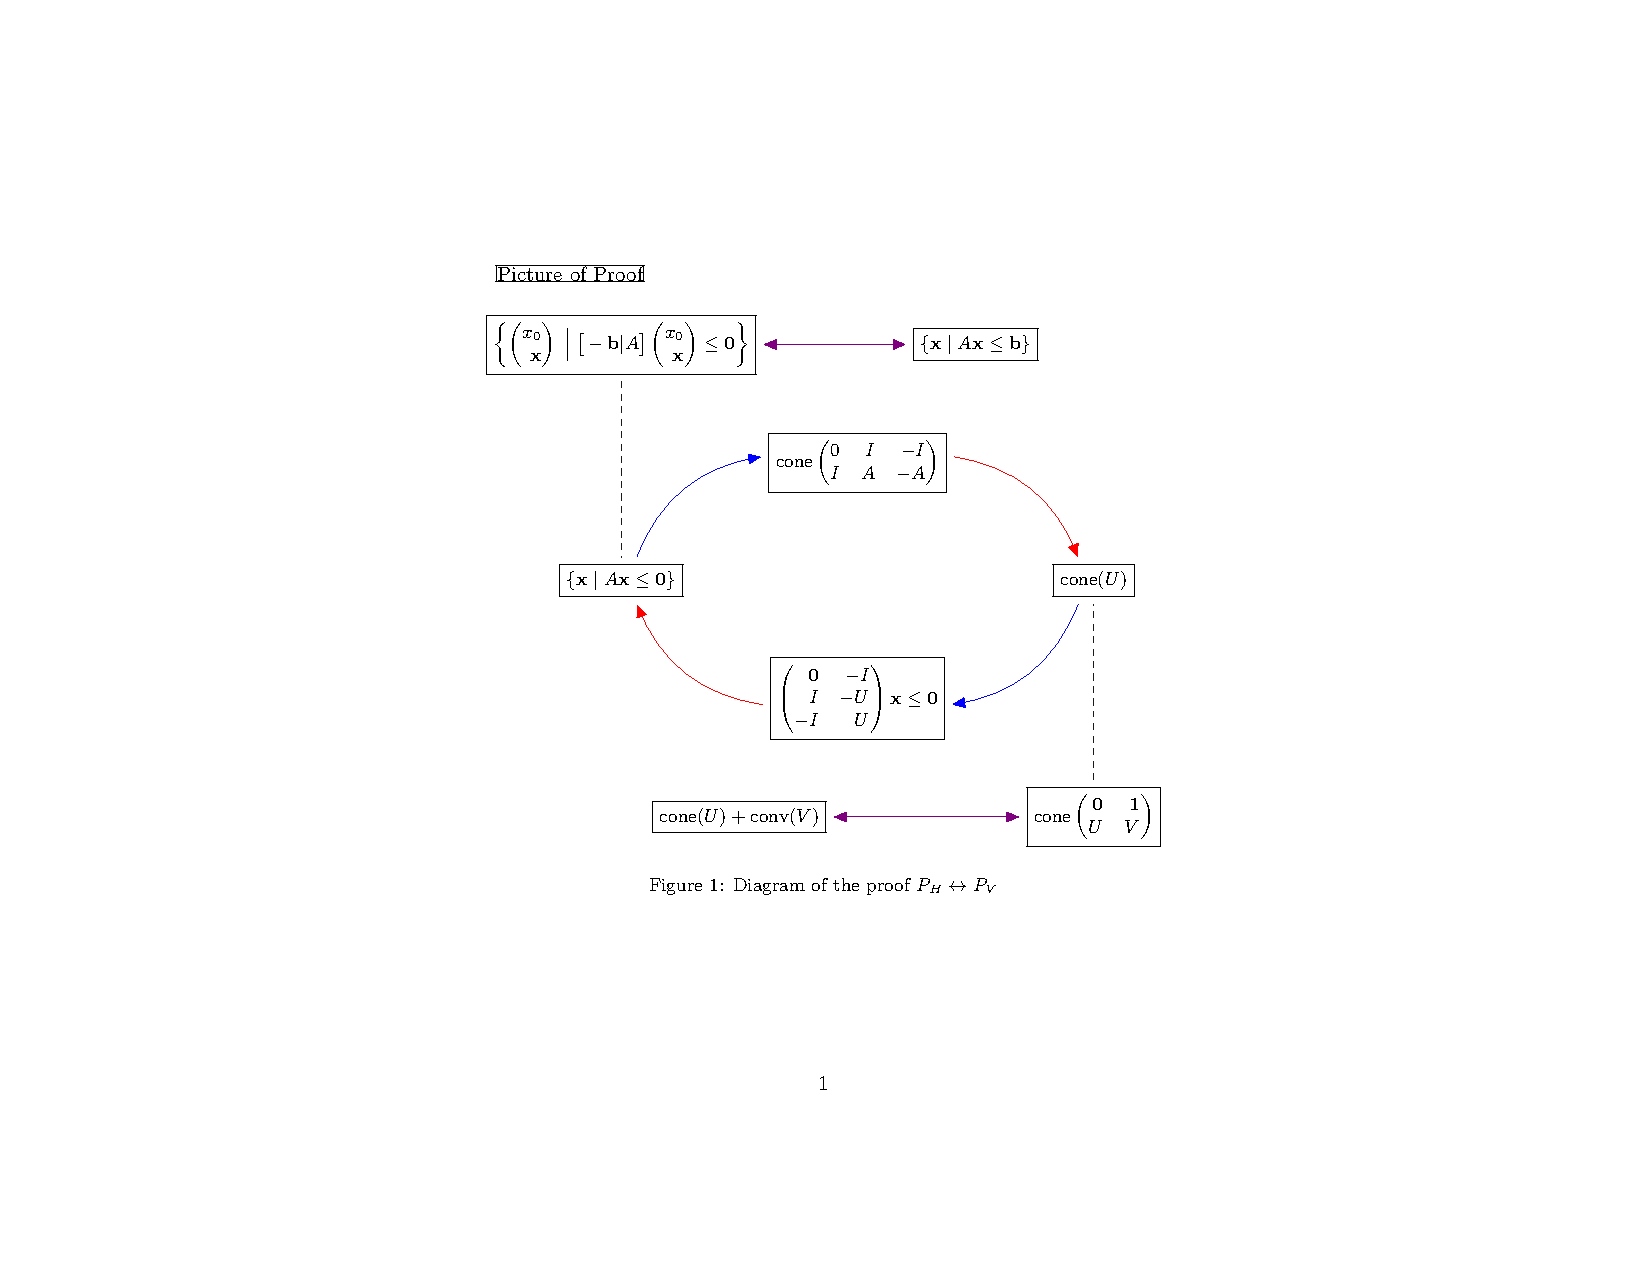
\includegraphics[width = {\picwidth}pt, trim=6cm 0 0 4cm, page=1]{proof_picture_landscape.pdf}
\end{frame}


%\subsection{"Original"}
%
%\begin{frame}
%\begin{itemize}
%  \item<1-> Some of the work and results are ``original''
%  \item<2-> I mean that I came up with them on my own, I'm sure they already exist somewhere
%  \item<3-> The implementation
%  \item<4-> The properties characterizing pointed and full-dimensional polyhedra and their proofs
%\end{itemize}
%\end{frame}

\subsection{Implementation}

\begin{frame}{Files and Includes}
	\begin{tabular}{|l|l|}
		\hline
		file                          & includes                                             \\
		\hline
		\filename{linear\_algebra.h}  & \filename{<C++ standard library>}                    \\
		\filename{fourier\_motzkin.h} & \filename{linear\_algebra.h}                         \\
		\filename{polyhedra.h}        & \filename{fourier\_motzkin.h}                        \\
		\filename{main.cpp}           & \filename{polyhedra.h}                               \\
		\hline
		\filename{test\_functions.h}  & \filename{linear\_alebra.h}                          \\
		\filename{test.cpp}           & \filename{test\_functions.h}, \filename{polyhedra.h} \\
		\hline
	\end{tabular}\\
\end{frame}

\begin{frame}{Callgraph}
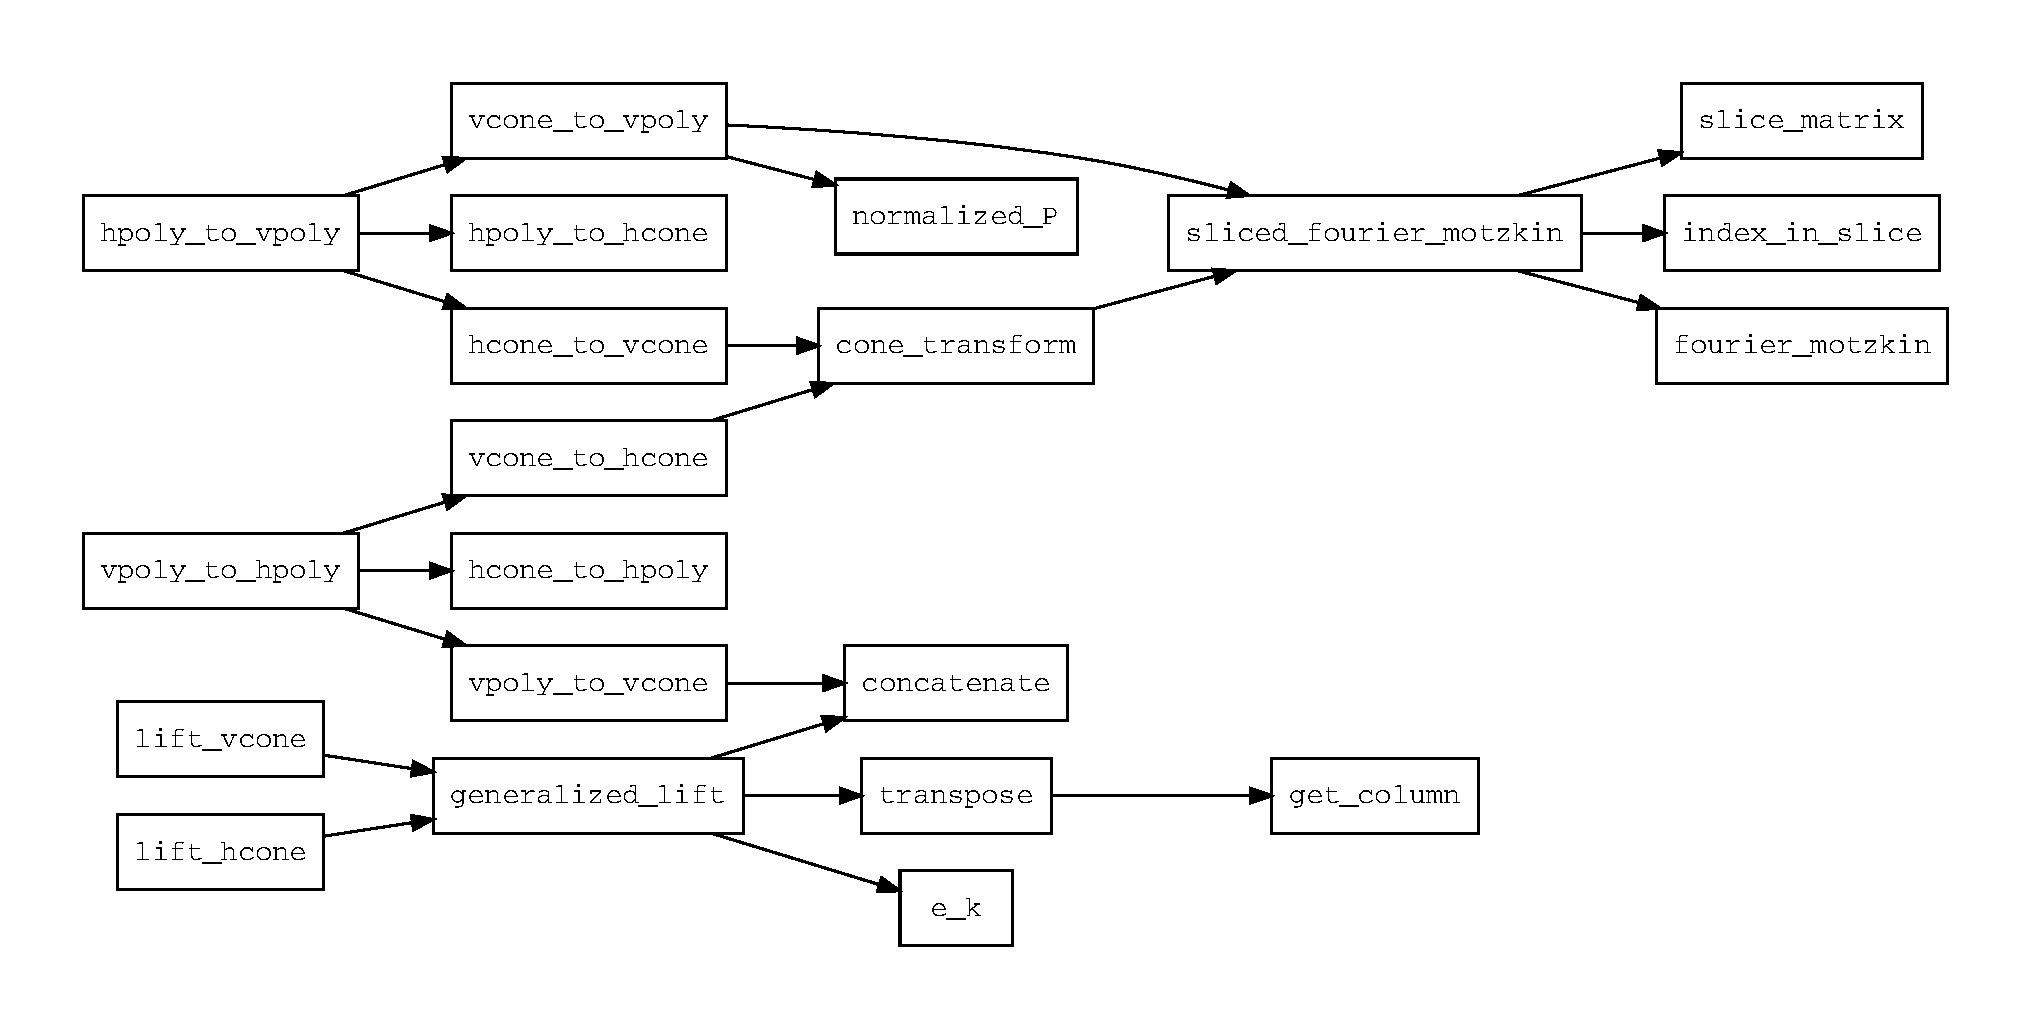
\includegraphics[angle=90, width=\textwidth]{../img/callgraph.pdf}
\end{frame}

\begin{frame}{{\tt Matrix fourier\_motzkin(Matrix,k)}}
\lstFMEPart
Partition \lsti{M} into logical sets $Z,P,N$ that satisfy the following:\\

\begin{tabular}{|l|l|l|}
	\hline
	set & range                               & property     \\
	\hline
	$Z$ & [\lsti{M.begin()}, \lsti{z_end} $)$ &
	\lsti{it} $\in Z \Leftrightarrow$ \lsti{(*it)[k]} $ = 0$ \\
	\hline
	$P$ & [\lsti{z_end}, \lsti{p_end} )       &
	\lsti{it} $\in P \Leftrightarrow$ \lsti{(*it)[k]} $ > 0$ \\
	\hline
	$N$ & [\lsti{p_end}, \lsti{M.end()})      &
	\lsti{it} $\in N \Leftrightarrow$ \lsti{(*it)[k]} $ < 0$ \\
	\hline
\end{tabular}\\
\end{frame}

\begin{frame}{{\tt Matrix fourier\_motzkin(Matrix,k)}}
\lstFMEConvolute
This function creates the sets which correspond to:

$\set{\Bik B_j - \Bjk B_i \st i \in P,\, j \in N}, \quad
	\set{\Yi Y^j - \Yj Y^i \st i \in P,\, j\in N} $
\end{frame}

\subsection{Pointed / Full-Dimensional Polyhedra}

\begin{frame}{Testing Methods}
\begin{itemize}
  \item<1-> Suppose we have an H-Cone $\HC{A}$, know that $\HC{A} = \cone(V)$, and would like to test if $\cone(V) = \cone(V')$
    \begin{alignat*}{2}
       & AV'\leq\0 \;      & \Rightarrow & \; \cone(V') \subseteq \HC{A}\\
       & V \subseteq V' \; & \Rightarrow & \; \cone(V) \subseteq \cone(V')\\
       & \cone(V') \subseteq \HC{A} \;   & \Rightarrow & \; AV'\leq\0 \\
       & \cone(V) \subseteq \cone(V')  \;& \overset{?}{\Rightarrow} & \; V \subseteq V'
    \end{alignat*}
  \item<2-> The last item would create an equivalence
  \begin{itemize}
    \item<3-> Must relax ``$\subseteq$'' (vectors vs rays)
    \item<4-> Requires notion of ``essentially unique'' representation
  \end{itemize}
\end{itemize}
\end{frame}

\begin{frame}{Pointed/ Full-Dimensional Polyhedra}
\begin{itemize}
  \item<1-> These are basically non-degeneracy constraints.
    \begin{itemize}
      \item<2-> Pointed Polyhedra have at least one vertex
      \item<3-> Full dimensional polyhedra contain an affine independent set
    \end{itemize}
  \item<4-> Pointed V-Polyhedra and Full-Dimensional H-Polyhedra have ``essentially unique'' sets of generators / contraints
  \item<5-> These ``essentially unique'' sets make it easy to test for equivalence
  \item<6-> The characterizations are similar to ``linear independence''
\end{itemize}
\end{frame}

\begin{frame}{Pointed/ Full-Dimensional Polyhedra}
\begin{itemize}
  \item<1-> These ``essentially unique'' sets are ``minimal''
  \item<2-> A set $V$ is called \textit{minimal} for $\cone(V)$ if
        \[ (\forall \vec{v}\in V)\; \cone(V\setminus\set{\vec{v}}) \subsetneq \cone(V) \]
  \item<3-> A set $A$ is called \textit{minimal} for $\HC{A}$ if
        \[ (\forall A_i \in A)\; \HC{A\setminus\set{A_i}} \supsetneq \HC{A} \]
  \item<4-> The definitions are similar for general polyhedra
\end{itemize}
\end{frame}

%\subsection{Cones}

\begin{frame}{Pointed V-Cones}
\begin{itemize}
  \item<1-> The following statements are equivalent.
    \begin{enumerate}
      \item $\cone(V)$ is pointed.
      \item $\t\geq\0,\; [V\t=\0 \Rightarrow \t=\0]$
    \end{enumerate}
  %\item<2-> A set $V$ is called \textit{minimal} for $\cone(V)$ if:\\
  %$(\forall \vec{v} \in V)\; \cone(V\setminus\{\vec{v}\}) \subset \cone(V)$
	\item<2-> Suppose that $\cone(V)$ is pointed.  The following two statements are equivalent:
	\begin{enumerate}
		\item V is minimal
		%\item $\t\geq\0,\,\vec{v}=V\e_i,\; [\vec{v}=V\t \Rightarrow \t=\e_i]$
		\item $\t\geq\0, [V\t = V\e_i \Rightarrow \t=\e_i]$
	\end{enumerate}
  \item<3-> ``No generator can be non-trivially generated''
\end{itemize}
\end{frame}

\begin{frame}{Farkas Lemma}
\begin{enumerate}
  \item<1-> Farkas Lemma:
    Let $U \in \R^{d\times n}$.  Precisely one of the following is true:
    \begin{align*}
       & (\exists \t \geq \0) : \x = U\t                \\
       & (\exists \y) : U^T\y \leq 0,\; \ip{\y}{\x} > 0
    \end{align*}
  \item<2-> i.e. a point is contained in a cone or can be separated from it with a hyperplane
\end{enumerate}
\end{frame}

\begin{frame}{Full-Dimensional H-Cones}
\begin{itemize}
  \item<1-> A set $V$ of vectors is \textit{full-dimensional} if 
  \[ \forall\y\neq\0, \forall c\in\R, \exists \vec{v} \in V:\; \y^T \vec{v} \neq c \]
  \item<2->The following two statements are equivalent:
    \begin{enumerate}
      \item $\HC{A}$ is full dimensional and $A$ is minimal
      \item $\cone(A^T)$ is pointed and $A$ is minimal
    \end{enumerate}
  \item<3-> The Farkas Lemma can be used to prove the following: 
    \[\HC{A} = \HC{A'} \Leftrightarrow \cone(A^T) = \cone(A'^T)\]
    ($\cone(A^T)$ is what I call the ``dual cone'')
\end{itemize}
\end{frame}

%\subsection{Polyhedra}

\begin{frame}{Cones and Polyhedra}
\begin{itemize}
  \item<1-> General polyhedra are decomposed into a ``characteristic-cone'' and polytope
  \item<2-> Suppose that $P = \HP{A}{b} = \VP{U}{V}$, and let $\vec{r}$ be a vector.  The following are equivalent:
    \begin{enumerate}
      \item $A\vec{r}\leq\0$
      \item $(\forall \vec{x}\in P)(\forall \alpha > 0)\;\vec{x} + \alpha\vec{r} \in P$
      \item $\vec{r} \in \cone(U)$
    \end{enumerate}
  \item<3-> $2 \Rightarrow 3$ requires the Farkas Lemma
  \item<4-> Note that $(2)$ in the proof above is independent of $A$ and $U$.
\end{itemize}
\end{frame}

\begin{frame}{Pointed V-Polyhedra}
\begin{itemize}
  \item<1-> Minimality for the set $\conv(V)$ -- a polytope -- is given by the vertex set
  \item<2-> In $P = \cone(U)+\conv(V)$ we need $U$ to be minimal as for V-Cones
  \item<3-> Complication: a vertex of $\conv(V)$ may not be a vertex of $P$
\end{itemize}
\end{frame}

\begin{frame}{Pointed V-Polyhedra}
\begin{itemize}
	\item<1-> If $\vec{v}$ is a vertex of $\VP{U}{V}$, then $[\vec{v} = U\vec{t} + V\blambda] \Rightarrow \vec{t} = \0$  \\
  (I call $\vec{v}$ here \textit{U-free})
  \item<2-> If $\vec{v}$ is a vertex of $\VP{U}{V}$, then $\vec{v}$ is a vertex of $\conv(V)$
	\item<3-> Let $P = \cone(U)+ \cone(V)$ be pointed.  The following are equivalent
    \begin{enumerate}
      \item $(U,V)$ is minimal for $P$
      \item $U$ is minimal for $\cone(U)$, $V$ is the vertex set of $P$
      \item $U$ is minimal for $\cone(U)$, $V$ is the vertex set of $\conv(V)$, and $V$ is $U$-free
    \end{enumerate}

\end{itemize}
\end{frame}

\begin{frame}{Farkas Lemma 2}
\begin{itemize}
  \item<1-> We need another form of the Farkas Lemma:
      \[ (\exists \vec{t}\geq\0) \vec{t}^T A = \vec{y},\, \vec{t}^T\vec{b} \leq c \Leftrightarrow
        \begin{cases}
        (\forall \vec{x}) A\vec{x}\leq \0 \Rightarrow \vec{y}^T\vec{x} \leq 0 \textbf{ and } \\
        (\forall \vec{x}) A\vec{x}\leq \vec{b} \Rightarrow \vec{y}^T\vec{x} \leq c
        \end{cases}
      \]
  \item<2-> Basically, a constraint is valid for a polyhedron if and only if it is a non-negative combination of rows of constraints (plus some change)
\end{itemize}
\end{frame}

\begin{frame}{Full-Dimensional H-Polyhedra}
\begin{itemize}
  \item<1-> The following are equivalent
  \begin{enumerate}
    \item $\HP{A}{\vec{b}}$ is full-dimensional
    \item $ \y\geq\0,\, \vec{y}^T A = \0 \Rightarrow 
      \vec{y} = \0 \text{ or } \vec{y}^T \vec{b} > \0 $
  \end{enumerate}
  \item<2-> $\vec{y}^T A = \0,\;\vec{y}^T \vec{b} > \0$ occurs when two of the bounding hyperplanes are parallel
  \item<3-> If $\HP{A}{\vec{b}}$ is full-dimensional, the following are equivalent
  \begin{enumerate}
    \item $(A,\vec{b})$ is minimal
    \item $\y\geq\0,\y\neq\e_i, \y^T A = A_i \Rightarrow \y^T\vec{b} > b_i$
  \end{enumerate}
  \item<4-> ``A non-trivially generated row generates a trivial constraint''
\end{itemize}
\end{frame}

\begin{frame}{Dual Homogenization Cone}
\begin{itemize}
  \item<1-> For H-Polyhedra switching to the dual setting is slightly more complicated
  \item<2-> 	The following two statement are equivalent:
    \begin{enumerate}
      \item $\HP{A}{\vec{b}} = \HP{A'}{\vec{b}'}$
      \item $\cone \pmb -\vec{b}^T & -1 \\ A^T & \0 \pme = \cone \pmb -\vec{b}'^T & -1 \\ A'^T & \0 \pme$
    \end{enumerate}
  \item<3-> If $\HP{A}{\vec{b}}$ is minimal and full-dimensional, then either 
    \begin{enumerate}
      \item $\cone \pmb -\vec{b}^T & -1 \\ A^T & \0 \pme$ is minimal and pointed, or
      \item $\cone \pmb -\vec{b}^T \\ A^T \pme$ is minimal and pointed, and $\cone\pmb -\vec{b}^T \\ A^T \pme = \cone \pmb -\vec{b}^T & -1 \\ A^T & \0 \pme$
    \end{enumerate}
\end{itemize}
\end{frame}

\begin{frame}{Pointed H-Polyhedra and Full-Dimensional V-Polyhedra}
\begin{itemize}
  \item $\vec{t}$ is a non-negative vector, $V \neq \emptyset$, and abbreviate {\LI} as LI. $\bar V$ denotes $\{\vec{v}-\vec{v}'\st\vec{v},\vec{v}'\in V\}$.\\

  \renewcommand{\arraystretch}{1.3}
  \resizebox{\columnwidth}{!}{
  \begin{tabular}{|l|l|l|}\hline
          & Pointed & Full-Dimensional \\ \hline
    $\cone(U)$ & $U\vec{t}=\0 \Rightarrow \vec{t}=\0$ & $d$ LI vectors in $U$ \\  \hline
    $\cone(U)+\conv(V)$ & $U\vec{t}=\0 \Rightarrow \vec{t}=\0$ & $d$ LI vectors in $U\cup \bar V$ \\ \hline
    $\HC{A}$ & $d$ LI row vectors in $A$ & $\vec{t}^T A=\0 \Rightarrow \vec{t}= \0$ \\ \hline
    $\HP{A}{\vec{b}}$ & $d$ LI row vectors in $A$ & $\vec{t}^T A=\0 \Rightarrow \vec{t}^T\vec{b} > 0$ \\ \hline
  \end{tabular}
  }
\end{itemize}
\end{frame}

\begin{frame}{Not much to see here}
\begin{itemize}
  \item The proofs are more tedious than enlightening
  \item The implementation is straightforward
\end{itemize}
\end{frame}


\section{Closing Remarks}

\subsection{If I could do it again}

%\begin{frame}{20/20 hindsight}
%\begin{itemize}
%  \item Since writing the thesis I've come up with a ``more elegant'' proof of the MWT for cones.  I would rather have used this proof, but here it is now
%  \item I've read a little about tensors, and think that using some of the ideas there and notation would have made things cleaner
%\end{itemize}
%\end{frame}

\begin{frame}{Better MWT for Cones}
\begin{itemize}
  \item H-Cone $\to$ V-Cone.  Use same transform and ``tensor-notation''
  \item Farkas Lemma using the following facts:
  \begin{enumerate}
    \item An intersection of closed sets is closed
    \item A projection of a closed subset of $\R^n$ is closed
    \item (Heine-Borel) A subset of $\R^n$ is compact if and only if it is closed
          and bounded
    \item A continuous function on a compact subset of $\R^n$ achieves its maximum
    \item Linear functions on $\R^n$ are continuous
    \item The Cauchy-Shwartz inequality
  \end{enumerate}
%  \begin{itemize}
%    \item Intersection of a closed set with a compact set is compact
%    \item Continuous real-valued function attains maximum on a compact set
%    \item Projection is bi-continuous on a finite product topology
%    \item Finitely generated cone is closed (project $V\to H$ transform)
%    \end{itemize}
  \item Better dual cone: $\HC{A} = \cone(U) \Leftrightarrow \cone(A^T) = \HC{U^T}$
\end{itemize}
\end{frame}

\begin{frame}{Tensor-like notation}
First, we write $\HC{A} = \set{ \vec{x} \St
    \pmb \vec{x} \\ \0 \pme \in 
      \cone \pmb I & -I & \0 \\ A & -A & I \pme }$
Now we need to do our intersections:
\begin{itemize}
  \item Let $\vec{u} \in \cone(U)$ with $u_l = 0$
  \item Let $\vec{p}^i t_i$ sum over elements of U with positive $l$-th elements
  \item $\vec{u} = \vec{p}^i t_i + \vec{n}^j t_j + \vec{z}^k t_k$
  \item $u_l = 0 \Rightarrow p^i_l t_i + n^j_l t_j = 0 \dots \quad \sigma := p^i_l t_i = -n^j_l t_j$
  \item $\vec{u} = \frac{\vec{n}^j t_j p^i_l t_i - \vec{p}^i t_i n^j_l t_j}{\sigma} + \vec{z}^k t_k = (\vec{n}^j p^i_l - \vec{p}^i n^j_l)\frac{t_i t_j}{\sigma} + \vec{z}^k t_k $
\end{itemize}
\end{frame}

\subsection{Summary}

\begin{frame}{Summary}
	% Keep the summary *very short*.
	\begin{itemize}
		\item<1-> Finite generation
		\item<2-> The Farkas Lemma (separation)
    \item<3-> Pointed and Full-Dimensional polyhedra are ``non-degenerate''
	\end{itemize}
\end{frame}

\begin{frame}{Further Considerations}
\begin{itemize}
  \item Better algorithms (Dual-Description)
  \item Other interpretations...
  \begin{itemize}
    \item ...Systems of logical deduction: \\
      Hahn-Banach vs Incompleteness
    \item ...Systems where ``lift and drop'' creates a dual representation
  \end{itemize}
  %\item Are there any useful implications for ``polyhedra complexes'' or ``chains''?
\end{itemize}
\end{frame}


%% All of the following is optional and typically not needed. 
%\appendix
%\section<presentation>*{\appendixname}
%\subsection<presentation>*{For Further Reading}
%
%\begin{frame}[allowframebreaks]
%	\frametitle<presentation>{For Further Reading}
%
%	\begin{thebibliography}{10}
%


%		\beamertemplatebookbibitems
%		% Start with overview books.
%
%		\bibitem{Author1990}
%		A.~Author.
%		\newblock {\em Handbook of Everything}.
%		\newblock Some Press, 1990.
%
%
%		\beamertemplatearticlebibitems
%		% Followed by interesting articles. Keep the list short. 
%
%		\bibitem{Someone2000}
%		S.~Someone.
%		\newblock On this and that.
%		\newblock {\em Journal of This and That}, 2(1):50--100,
%		2000.
%	\end{thebibliography}
%\end{frame}
%

\end{document}
